\documentclass{snapshotmfo}

\categorizationmath{algebra and number theory,analysis,discrete mathematics and foundations,geometry and topology,numerics and scientific computing,probability theory and statistics} %at least one must be chosen. 
\categorizationconnect{chemistry and earth science,computer science,engineering and technology,finance,humanities and social sciences,life science,physics,reflections on mathematics} %can be void.
\license{CC-BY-SA-4.0} %recommended
\snapshotid{136}{1950}
\junioreditor{Some One}{junior-editors@mfo.de}
\senioreditor[f]{Carla Cederbaum}{senior-editor@mfo.de}
\director[m]{Gerhard Huisken}

%%% Commands for editing
% Uncomment for collaborative editing:
\usepackage{trackchanges}
\addeditor{Alice}
\addeditor{Bob}
\addeditor{Carol}
\addeditor{Dave}

\usepackage[utf8]{inputenc}
\usepackage{amsmath,amssymb}

%\usepackage[ngerman]{babel}
\usepackage[USenglish]{babel}

\author{Author One\thanks{Author One is supported by the Mathematical Dreams Come True Foundation.} \and Author Two}

\title{trackchanges}

\authorinfo{\authorname{Author One} is a professor of pure mathematics at the First University.}
\authorinfo{\authorname{Author Two} is a lecturer in applied mathematics at the Second Institution.}

\usepackage{filecontents}
\begin{filecontents}{\jobname.bib}
@book{knuth1984texbook,
  title = {The TeXbook},
  author = {Knuth, D. E.},
  year = {1984},
  edition={1},
  publisher = {Addison-Wesley}
}

@misc{wikiMath,
  author = {Wikipedia},
  title = {Mathematics --- {W}ikipedia{,} The Free Encyclopedia},
  year = {2014},
  url = {https://en.wikipedia.org/wiki/Mathematics},
  urldate = {2014-05-19}
}

@misc{sample13,
  author = {Sample, J.},
  howpublished = {\href{http://arxiv.org/abs/8765.4321v1}{arxiv:8765.4321v1}},
  title = {Interesting facts in mathematics},
  year = {2013}
}

@incollection{sample12,
  author = {Sample, J.},
  title = {Things you don't know about mathematics},
  booktitle = {A bookseries about mathematics},
  publisher = {Some publisher},
  year = {2012}
}

@inproceedings{sample11,
  author={Example, C.},
  title={A new perspective on mathematics},
  booktitle={New perspectives on arts and sciences},
  year={2011}
}

@phdthesis{sample14,
  author={Candidate, A.},
  title={Thesis title},
  school={MFO},
  year={2014}
}
\end{filecontents}
%%%%%%%%%%%%%%%%%%%%%%%%%%%%%%%%%%%%%%%%%%%%%%%%%%%%%%%%%%%%%%%%%%%%%%%%%%%%%%%%%%%%%%%%%%%%%%%%%%%%%%%%%%


%%%%%%%% If your latex file does not compile, please delete all .aux and .log files and try again. %%%%%%%
\begin{document}

%%% Please insert your abstract here. 
\begin{abstract}
Does the style file trackchanges.sty for collaborative editing work as expected?
\end{abstract}

\section{Comment on this unit test}
The snapshot template has been interspersed with editing by Alice, Bob, Carol, and Dave. Look for colors and footnotes.

Ordinary footnotes and trackchanges footnotes both are numbered consecutively, but independently of each other,
througout the whole document as 1, 2, 3, \dots\ and c1, c2, c3, \dots, respectively.
See test-hyperref.tex for footnotes in special places like section headings.

Latex should write the line
\begin{verbatim}
trackchanges.sty    2015/11/07 v0.7.2 TrackChanges file 
\end{verbatim}
with this date and version number to standard output. Otherwise latex has not loaded the version
adapted to the snapshotmfo.cls by Johannes Niediek.

%%% Please insert the main body of your snapshot here.
\section{A heading}
Your actual snapshot.\footnote{This is a footnote.} As usual, you can give references such as \cite{knuth1984texbook, wikiMath, sample13, sample12, sample11, sample14} via the \verb+\cite+ command.

\change[Alice]{We appreciate if you include images or other graphics that illustrate your snapshot. However, please do keep in mind the copyright issues explained in our email in case you include images and graphics you have not produced yourself.}{Lorem ipsum dolor sit amet, consetetur sadipscing elitr, sed diam nonumy eirmod tempor invidunt ut labore et dolore magna aliquyam erat, sed diam voluptua. At vero eos et accusam et justo duo dolores et ea rebum. Stet clita kasd gubergren, no sea takimata sanctus est Lorem ipsum dolor sit amet.}

%%% Please use this format to include images. Supported image formats: jpg, pdf, png. Please convert your images to those formats.
\begin{figure}[ht]
        \centering 
        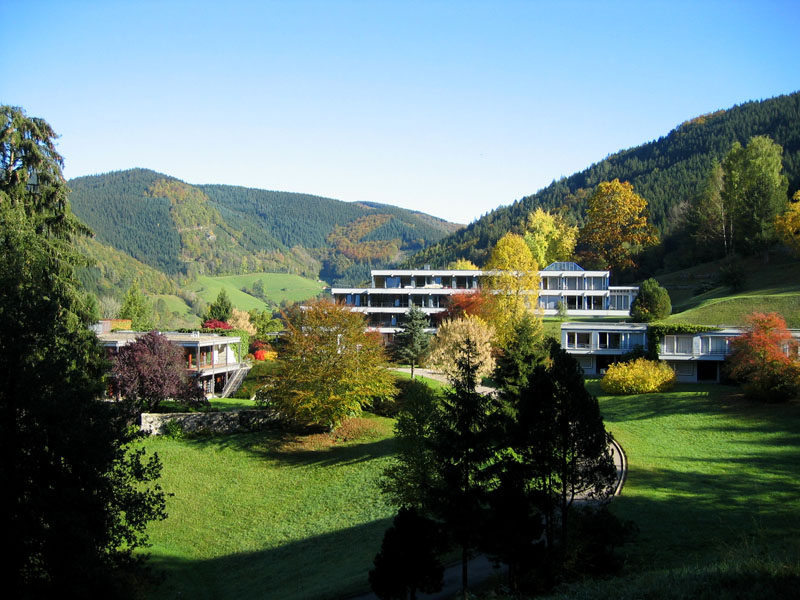
\includegraphics[width= 0.33 \textwidth]{mfo.jpg}
        \caption{An image scaled to 33\% of the textwidth.}
\label{fig:sample-image}
\end{figure}

\subsection{A subsection}
More text and some formulas:
\begin{align}\label{real}
1+1&=2,\\\label{char.2}
1+1&=0.
\end{align}
Formula \eqref{real} refers to $\mathbb{R}$, Formula \eqref{char.2} does not.

\section{More information}
We have composed guidelines to help you write a beautiful and accessible snapshot which you can download at \href{http://www.mfo.de/snapshots/guidelines-for-snapshots}{www.mfo.de/snapshots/guidelines-for-snapshots}. For more information on the snapshot project (including example snapshots), please see \href{http://www.mfo.de/snapshots}{www.mfo.de/snapshots}.

\add[Bob]{Sed diam nonumy eirmod tempor invidunt ut labore et dolore magna aliquyam erat, sed diam voluptua. At vero eos et accusam et justo duo dolores et ea rebum.} 

%%% Please use this format to include images. Supported image formats: jpg, pdf, png. Please convert your images to those formats.
\begin{figure}[ht]
        \centering 
        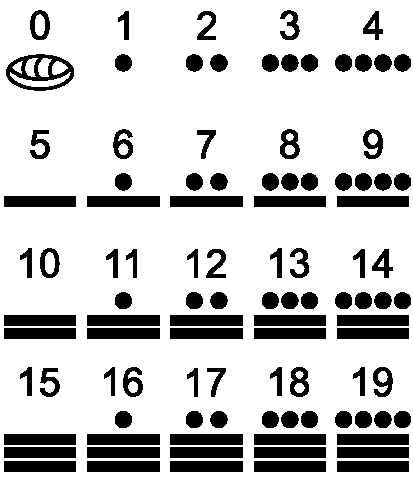
\includegraphics[width= 0.33 \textwidth]{maya.pdf}
        \caption{Exemplary image: Maya numerals.}
\label{fig:maya}
\end{figure}

If you download an image from Wikipedia\remove[Dave]{ or similar sources}, please always check the applicable license terms. Most licenses require an adequate attribution. For Wikipedia, you can find the correct reference by clicking on the image and then clicking on the button saying 'use this file‘. Some licenses may have further restrictions, such as 'modifications are not allowed'. If modifications\note[Alice]{Stet clita kasd gubergren, no sea takimata sanctus est.} are allowed you may still have to mark those modifications. Please verify that you comply with all license requirements.

If you use your own images, please check if you still have the rights of use. \annote[Carol]{The images may be copyrighted}{At vero eos et accusam et justo duo dolores et ea rebum.} by your institution or a publisher of your previous publications.

\clearpage

%%% Image credits: If you download an image form Wikipedia or similar sources, please always check the applicable license terms. Most licenses require an adequate attribution. For Wikipedia, you can find the correct reference by clicking on the image and then clicking on the button saying 'More details' and then on the link 'use this file' or similar. Some licenses may have further restrictions, such as 'modifications are not allowed'. If modifications are allowed you may still have to mark those modifications. Please verify that you comply with all license requirements. If you use your own images, please check if you still have the rights of use. The images may be copyrighted by your institution or a publisher of your previous publications.
\begin{imagecredits}
  \item[\autoref{fig:sample-image}] Archives of the Mathematisches Forschungsinstitut Oberwolfach,\\\url{http://www.mfo.de}, 2004.
  \item[\autoref{fig:maya}] ``Maya''. Author: Bryan Derkson. Licensed under Creative Commons Attribution-Share Alike 3.0 via Wikimedia Commons, \url{http://commons.wikimedia.org/wiki/File:Maya.svg}, visited on September 5, 2014.
\end{imagecredits}

\bibliography{\jobname}

\end{document}
